\documentclass{article}
\usepackage[utf8]{inputenc}
\usepackage[T1]{fontenc}
\usepackage[utf8]{inputenc}
\usepackage{lmodern}
\usepackage[greek]{babel}
\usepackage[a4paper, margin=1in]{geometry}
\usepackage{parskip}
\usepackage{amsmath}
\usepackage{forest}
\usepackage{graphicx}


\usepackage{minted}
\large
\title{Educational Software Assignment}
\begin{document}
\begin{titlepage}
	\begin{center}
    \line(1,0){300}\\
    [0.65cm]
	\huge{\bfseries Απαλλακτική Εργασία}\\
	\line(1,0){300}\\
	\textsc{\Large Εκπαιδευτικό λογισμικο}\\
    \textsc{\Large Τμήμα Πληροφορικής, Πανεπιστήμιο Πειραιώς}\\
	\textsc{\LARGE \today}\\
	[5.5cm]
	\end{center}
	\begin{flushright}
		\textsc{\Large Κατσιμίχα Ελένη\\Π21053}\\
		[0.5cm]
		\textsc{\Large Μπαρλάς Παύλος-Ιάσων\\Π21111}\\
		[0.5cm]
	\end{flushright}
\end{titlepage}

\tableofcontents
\newpage


\section{Εισαγωγή}
Στο πλαίσιο της παρούσας εργασίας αναπτύχθηκε η εφαρμογή \foreignlanguage{english}{GitGud}, η οποία αποτελεί εκπαιδευτικό λογισμικό για την εκμάθηση του συστήματος ελέγχου εκδόσεων \foreignlanguage{english}{(Version Control System) Git}. Σύμφωνα με το \foreignlanguage{english}{Stack Overflow Developer Survey} του 2022, το \foreignlanguage{english}{Git} χρησιμοποιείται από το 93.87\%
των ερωτηθέντων, ενώ αποτελεί το πιο διαδεδομένο σύστημα ελέγχου εκδόσεων. Για ένα εργαλείο με τόσο μεγάλο ποσοστό αξιοποίησης, η εξοικείωση με τη χρήση του αποτελεί σημαντική δεξιότητα για τους \foreignlanguage{english}{developers}. Ωστόσο, η εκμάθηση και η χρήση του \foreignlanguage{english}{Git} μπορεί να παρουσιάσει σημαντικές δυσκολίες, ιδιαίτερα για τους αρχάριους χρήστες. Έρευνες έχουν εντοπίσει προκλήσεις και συγχύσεις κατά την εκμάθηση και τη χρήση του \foreignlanguage{english}{Git}, όπως με τα “\foreignlanguage{english}{branches}”, τα οποία έχουν αναδειχθεί ως σημαντική γνωστική πρόκληση για τους αρχάριους χρήστες \foreignlanguage{english}{(Jansson, 2013)}. Συνεπώς, κρίθηκε αναγκαία η επιλογή του \foreignlanguage{english}{Git} ως η θεματική ενότητα της εφαρμογής.

Το λογισμικό απευθύνεται σε αρχάριους χρήστες του \foreignlanguage{english}{Git}, οι οποίοι έχουν προηγούμενη εξοικείωση με τη χρήση ηλεκτρονικού υπολογιστή και στοιχειώδεις γνώσεις προγραμματισμού. Το υλικό της εφαρμογής είναι στα Αγγλικά. Επιπλέον, το \foreignlanguage{english}{visual design/ front end} της εφαρμογής εμπνεύστηκε κυρίως από τη διαδικτυακή πλατφόρμα μάθησης “\foreignlanguage{english}{W3SCHOOLS}”.


Μέσω της εφαρμογής, οι χρήστες μαθαίνουν για τις βασικές και προχωρημένες έννοιες του \foreignlanguage{english}{Git}, μέσα από τρία κεφάλαια δομημένου εκπαιδευτικού υλικού και διαδραστικών ασκήσεων αξιολόγησης.

\newpage

\section{Θεωρία Μάθησης}
Για την ανάπτυξη του εκπαιδευτικού λογισμικού αξιοποιήθηκε η Συμπεριφοριστική Θεωρία Μάθησης \foreignlanguage{english}{(Behaviorism)}, όπως αναπτύχθηκε από τους \foreignlanguage{english}{John Watson} και \foreignlanguage{english}{B.F. Skinner}, μεταξύ άλλων. Σύμφωνα με αυτή τη θεωρία, “οι συμπεριφορές είναι αποτελέσματα εξωτερικών ερεθισμάτων και οι μαθητές ανταποκρίνονται σε συγκεκριμένα ερεθίσματα” (\foreignlanguage{english}{Kontogianni, 2024)}. Συνεπώς, η μάθηση είναι αποτέλεσμα της σχέσης μεταξύ των ερεθισμάτων και αποκρίσεων του μαθητή. Στην πράξη, αυτή η σχέση εδραιώνεται μέσω της άμεσης ανατροφοδότησης (\foreignlanguage{english}{immediate reinforcement)}, που προκύπτει από τις εκπαιδευτικές ερωτήσεις/ δραστηριότητες. Πιο συγκεκριμένα, στο εκπαιδευτικό λογισμικό υπάρχουν τρία διαφορετικά είδη ερωτήσεων, τα οποία απαρτίζουν οι ερωτήσεις πολλαπλής επιλογής, ερωτήσεις συμπλήρωσης κενών και ερωτήσεις σωστού-λάθους. Οι εκπαιδευτικές ενότητες έχουν σχηματιστεί ώστε να είναι \foreignlanguage{english}{"bite sized"}, και στο τέλος κάθε ενότητας υπάρχει ένα \foreignlanguage{english}{Quiz}, που περιέχει τα τρία ήδη ερωτήσεων που προαναφέρθηκαν. Με την ολοκλήρωση του κάθε \foreignlanguage{english}{Quiz}, ο μαθητής πληροφορείται αν οι απαντήσεις του είναι σωστές η λανθασμένες.

Η εφαρμογή στοχεύει στην συστηματική επανάληψη. Αυτό επιτυγχάνεται με την χρήση τριών διαφορετικών ειδών \foreignlanguage{english}{Quiz} που αντιστοιχούν στο \foreignlanguage{english}{QuizType}. To \foreignlanguage{english}{Practice Quiz} βρίσκεται στο επίπεδο κάθε υποενότητας και επιτρέπει την άμεση εξάσκηση του μαθητή. Το \foreignlanguage{english}{Final Quiz} βρίσκεται στο επίπεδο του κεφαλαίου και αξιολογεί τη συνολική κατανόηση της ύλης, ενώ το \foreignlanguage{english}{Review Quiz} περιέχει ερωτήσεις από όλα τα κεφάλαια. Ο διαχωρισμός αυτός εξασφαλίζει ότι ο μαθητής θα συναντήσει τις ίδιες ερωτήσεις πολλαπλές φορές, πράγμα που ενισχύει την μακροπρόθεσμη απομνημόνευση των εννοιών (\foreignlanguage{english}{spaced repetition)}.

Κάθε ερώτηση χαρακτηρίζεται από επίπεδο δυσκολίας \foreignlanguage{english}{(easy, medium, hard)} μέσω του \foreignlanguage{english}{QuestionDifficulty}. Η προσέγγιση αυτή καθοδηγεί σταδιακά τον μαθητή από απλές σε όλο και πιο σύνθετες ερωτήσεις. Ο μαθητής χτίζει αυτοπεποίθηση με τις εύκολες ερωτήσεις, προτού αντιμετωπίσει πιο δύσκολα σενάρια στις ερωτήσεις. Με αυτόν τον τρόπο, μειώνεται η πιθανότητα της απογοήτευσης και της εγκατάλειψης της διδακτικής διαδικασίας.

Επιπροσθέτως, για την κάθε ερώτηση έχουν προστεθεί δυο επίπεδα υποδείξεων \foreignlanguage{english}{(hints)}, τα οποία αποκαλύπτονται βαθμιαία. Οι υποδείξεις δρουν ως ενδιάμεσα ερεθίσματα, και καθοδηγούν τον μαθητή προς την σωστή απάντηση. Ο αριθμός των υποδείξεων που χρησιμοποιήθηκαν καταγράφεται στο \foreignlanguage{english}{QuestionAttempt (hintsUsed)}, για την αξιολόγηση του γνωστικού επιπέδου του μαθητή.

Για κάθε απάντηση του χρήστη αποθηκευονται στην \foreignlanguage{english}{QuestionAttempt} η ορθότητα της απάντησης \foreignlanguage{english}{(correct)}, ο χρόνος που αφιερώθηκε \foreignlanguage{english}{(timeSpentMillis)} ο αριθμός των υποδείξεων \foreignlanguage{english}{(hintsUsed)} και ο αριθμός των παραλήψεων \foreignlanguage{english}{(skipCount)}. Τα δεδομένα αυτά επιτρέπουν την ανάλυση της προόδου του χρήστη.

\newpage
\section{Εκπαιδευτική Διαδικασία}
Η εφαρμογή περιλαμβάνει τρία εκπαιδευτικά κεφάλαια, με τίτλους \foreignlanguage{english}{“What is Git?, Why use it?”, “Introduction to git Branches and Merging”} και \foreignlanguage{english}{“Remote Repositories”}. Η κάθε ενότητα και το κάθε κεφάλαιο περιλαμβάνει ένα αντίστοιχο \foreignlanguage{english}{Quiz}. Η επιτυχής ολοκλήρωση του \foreignlanguage{english}{Quiz}, αποτελεί προϋπόθεση για το ξεκλείδωμα της επόμενης ενότητας ή του επόμενου κεφαλαίου.

Κάθε \foreignlanguage{english}{Quiz} που είναι αποθηκευμένο στην \foreignlanguage{english}{Firestore} περιλαμβάνει έναν αριθμό ερωτήσεων διαφορετικού επιπέδου δυσκολίας. Οι ερωτησεις κατανέμονται ισόποσα μεταξύ των διαθέσιμων επιπέδων δυσκολίας, τα οποία διακρίνονται σε εύκολες, μέτριας δυσκολίας και δύσκολες ερωτήσεις.

Σε κάθε προσπάθεια επίλυσης που προβαίνει ο χρήστης, πρεπει να απαντήσει σε πέντε ερωτήσεις. Η επιλογή των ερωτήσεων επηρεάζεται από την κατηγορία του χρήστη/ ή και την βαθμολογια κατάταξής του. Έτσι η πιθανοτητα εμφάνισης ερωτήσεων μίας συγκεκριμένης κατηγορίας προσαρμόζεται στο επίπεδο του χρήστη. Λόγου χάριν, ένας χρήστης που θεωρείται αρχάριος έχει μεγαλύτερη πιθανότητα να λάβει ευκολες ερωτήσεις, ενώ ένας χρήστης που θεωρείται έμπειρος έχει μεγαλύτερη πιθανότητα να λάβει δύσκολες ερωτήσεις.

Η επίδοση του χρήστη σε κάθε προσπάθεια αξιολογείται βάση του αριθμού των σωστών απαντήσεων, όπως περιγράφεται στην αμέσως επόμενη ενότητα.

\subsection{Προσδιορισμός κατηγορίας του χρήστη}
Κάθε ολοκληρωμένη προσπάθεια σε ένα \foreignlanguage{english}{Quiz} αποδίδει μία από τις παρακάτω βαθμολογίες επίδοσης:
\begin{enumerate}
    \item 0-2/5 σωστές απαντήσεις: \foreignlanguage{english}{Failure} (αποτυχία)
    \item 3/5 σωστές απαντήσεις: \foreignlanguage{english}{Passing} (επιτυχία)
    \item 4/5 σωστές απαντήσεις: \foreignlanguage{english}{Excellent} (εξαιρετικά)
    \item 5/5 σωστές απαντήσεις: \foreignlanguage{english}{Perfect} (άριστα)
\end{enumerate}

Για την αξιοποιηση των επιδόσεων των χρηστων στα \foreignlanguage{english}{Quiz} ως μέσο αξιολόγησης της συνολικής τους ικανότητας, δημιουργήθηκε ένα σύστημα παρόμοιο με τα συστήματα του \foreignlanguage{english}{ELO (chess)} και \foreignlanguage{english}{MMR (video games)}. Το σύστημα αποσκοπεί στον προσδιορισμό του κατά πόσο ένας χρηστης θεωρείται έμπειρος ή αρχάριος. Αυτο επιτυγχάνεται από την συνέπεια της απόδοσης του. Δηλαδή ο χρήστης θα μπορεί να αλλάξει κατηγορία, παραδείγματος χάριν από αρχάριος σε προχωρημένος, μέσω σταθερά καλών επιδόσεων.

\subsection{Τρόπος βαθμολόγησης}
Κάθε ολοκληρωμένη προσπάθεια σε ένα \foreignlanguage{english}{Quiz} αποδίδει μια βαθμολογία. Η βαθμολογία αυτή αντικαθίσταται μόνο όταν κάποια μεταγενέστερη προσπάθεια αποφέρει υψηλότερη βαθμολογία, ενώ η τελική βαθμολογία υπολογίζεται λαμβάνοντας υπόψιν την δυσκολία των ερωτήσεων, τη χρήση υποδείξεων \foreignlanguage{english}{(hints)}, τις παραλήψεις \foreignlanguage{english}{(skip for now)}, και τον χρόνο που χρειάστηκε για την εκάστοτε απάντηση. Ενδεικτικά:

Για την βαθμολογία του \foreignlanguage{english}{Quiz} έστω ότι:

\begin{itemize}
    \item $G$ = \foreignlanguage{english}{base} βαθμός ερώτησης
    \item $D$ = συντελεστής δυσκολίας
    \item $H$ = αριθμός χρησιμοποιημένων υποδείξεων
    \item $S$ = αριθμός των παραλείψεων
    \item $T$ = χρόνος απάντησης σε δευτερόλεπτα
    \item  $P$ = ποινή ανά παράλειψη
\end{itemize}

Ο συντελεστής δυσκολίας για μία ερώτηση $i$ ορίζεται ως:

\[D_i = \begin{cases}
2, & \text{εύκολη ερώτηση} \\
3, & \text{ερώτηση μέτριας δυσκολίας} \\
4, & \text{δύσκολη ερώτηση}
\end{cases}\]

Η βαθμολογία μιας σωστής απάντησης πριν τις ποινές υπολογίζεται ως:

\[Q_{\mathrm{correct}, i} = G_i \cdot D_i\]

Η χρήση υποδείξεων αντιστοιχεί σε ποινή της τάξης του $10\%$ για κάθε υπόδειξη που χρησιμοποιήθηκε. Επομένως:

\[
P_{\mathrm{hint}, i} = Q_{\mathrm{correct}, i} \cdot 0.10 \cdot H_i
\]

Η ποινή για τις παραλήψεις υπολογίζεται ως:

\[
P_{\mathrm{skipped}, i} = P \cdot S_i
\]

Για κάθε επιπλέον δευτερόλεπτο (ξεκινώντας από το $6^\mathrm{o}$) εφαρμόζεται ποινή της τάξης του $2\%$ επί της αρχικής βαθμολογίας της ερώτησης:

\[
P_{\mathrm{time}, i} =
\begin{cases}
    0, & T_i \leq 5 \\
    0.02 \cdot (T_i -5) \cdot Q_{\mathrm{correct}, i}, & T_i >5
\end{cases}
\]

Επομένως η τελική βαθμολογία μιας ερώτησης μπορει να εκφραστεί ως:
\[
Q_{\mathrm{final},i}
=
\max\left(
0,\,
Q_{\mathrm{correct},i}
-
P_{\mathrm{hint},i}
-
P_{\mathrm{skipped},i}
-
P_{\mathrm{time},i}
\right)
\]

Και η συνολική βαθμολογία του \foreignlanguage{english}{Quiz} το οποίο αποτελείται από $5$ ερωτήσεις υπολογίζεται ως

\[
Score_{\mathrm{quiz}} = \sum_{i=1}^{5} Q_{\mathrm{final}, i}
\]

Τέλος, η βαθμολογία της προσπάθειας (\foreignlanguage{english}{attempt}) ορίζεται ως:

\[
Score_{\mathrm{attempt}} =
\begin{cases}
    0, & \text{αν ο χρήστης ακυρώσει το \foreignlanguage{english}{Quiz}} \\
    Score_{\mathrm{quiz}}, & \text{αν το \foreignlanguage{english}{Quiz} ολοκληρωθει}
\end{cases}
\]

Η μεγαλύτερη βαθμολογική αξία των δυσκολότερων ερωτήσεων χρησιμοποιείται για τον προσδιορισμό της κατηγορίας ενός χρήστη, καθως και για την συλλογή στατιστικών στοιχείων. Η βαθμολογια δεν χρησιμοποιείται για την προοδο του χρήστη μέσα στο εκπαιδευτικό περιεχόμενο. Ως αποτέλεσμα οι εμπειροι χρήστες έχουν την δυνατότητα να συγκεντρώνουν υψηλότερες βαθμολογίες, καθώς είναι πιθανότερο να αντιμετωπίσουν ερωτήσεις αυξημένης δυσκολίας.

\subsection{Βαθμολογία Κατάταξης}

Για να τοποθετηθεί ο χρήστης σε μία απο τις κατηγορίες, θα πρεπει να απαντησει στο εισαγωγικό \foreignlanguage{english}{Quiz}. Αν ο χρήστης απαντήσει σωστα σε $0-3/5$ θα λάβει την κατηγορία “αρχάριος”, ενώ σε κάθε άλλη περίπτωση θα λάβει την κατηγορία “έμπειρος”
Η βαθμολογία κατάταξης παραμένει κρυφή από τον χρήστη. Υπολογίζεται με βάση την απόδοσή του σε σχέση με την απόδοση που αναμένεται να έχει. \foreignlanguage{english}{(expected performance)}. Γενικά, από έναν αρχάριο χρήστη αναμένεται να έχει \foreignlanguage{english}{score} $0-3/5$, ενώ από έναν προχωρημένο χρήστη $4-5/5$.

\subsection{Επαναλαμβανόμενες προσπάθειες}
Ένας παράγοντας που θα μπορουσε να επηρεάσει αρνητικα την αξιοπιστία του συστήματος αυτου είναι η επανειλημμένη προσπάθεια του ίδιου \foreignlanguage{english}{Quiz}. Στην περίπτωση που ο χρήστης μπορεί να επαναλαμβάνει ένα \foreignlanguage{english}{Quiz} (απεριόριστες φορές), θα μπορούσε να βελτιώνει τεχνητά την βαθμολογία του, χωρίς να αντικατοπτρίζει απαραίτητα την συνολική επίδοσή του.
Λόγω αυτού, τα \foreignlanguage{english}{Quiz} των ενοτήτων και των κεφαλαίων επηρεάζουν τη βαθμολογία κατάταξης μόνο μία φορά ανά \foreignlanguage{english}{Quiz}, ενώ μετά το ξεκλείδωμα όλου του εκπαιδευτικου περιεχομένου, ο χρήστης αποκτά πρόσβαση στα επαναληπτικα \foreignlanguage{english}{Quiz}, τα οποία μπορούν να πραγματοποιηθούν πολλές φορές, και να χρησιμοποιηθούν για την περαιτέρω αξιολόγηση και μεταβολή της κατηγορίας του. Επιπλέον, κάθε ακυρωμένη προσπάθεια στο \foreignlanguage{english}{Quiz} υπολογίζεται ως μια επιπλέον αποτυχία στο σύστημα.


\begin{figure}[htp]
    \centering
    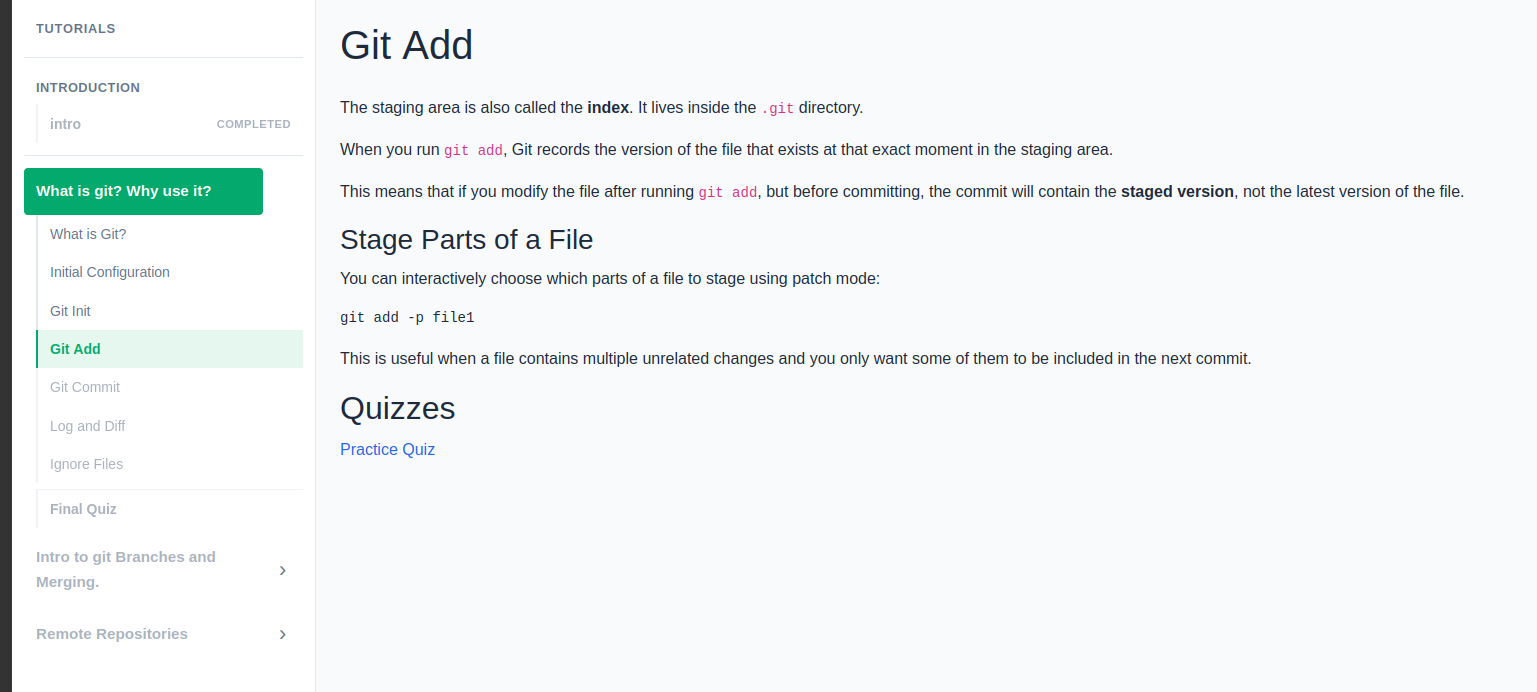
\includegraphics[width=15cm]{images/lesson.png}
    \caption{Μάθημα υποενότητας προχωρημένου χρήστη για το \foreignlanguage{english}{Git Add}}
    \label{fig:lesson}
\end{figure}

\begin{figure}[htp]
    \centering
    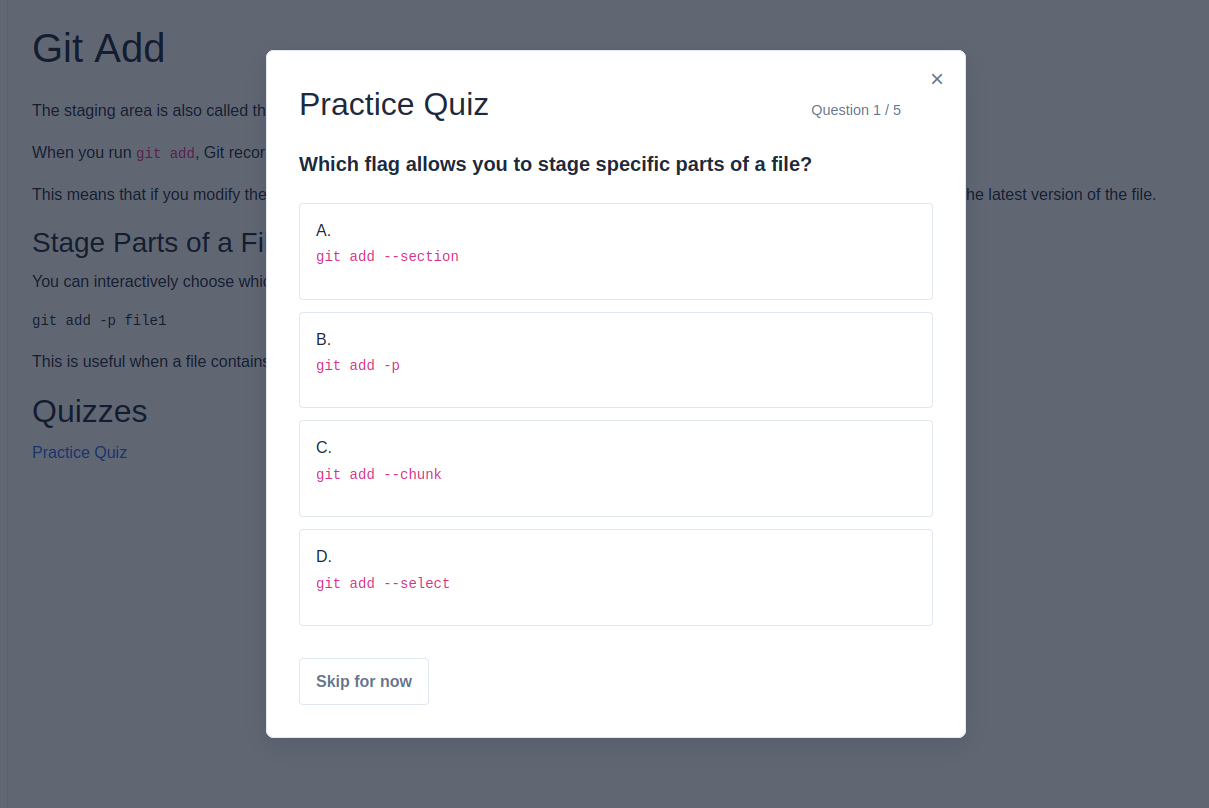
\includegraphics[width=15cm]{images/questions.png}
    \caption{\foreignlanguage{english}{Quiz} της υποενότητας \foreignlanguage{english}{Git add}, για τον προχωρημένο χρήστη}
    \label{fig:lesson}
\end{figure}

\section{\foreignlanguage{english}{Tech Stack}}
Η εφαρμογή είναι γραμμένη σε \foreignlanguage{english}{Java}, και έχει χτιστεί πάνω στο \foreignlanguage{english}{Spring Boot}, ως \foreignlanguage{english}{back end framework}. Επιπλέον, χρησιμοποεί \foreignlanguage{english}{Thymeleaf} στο \foreignlanguage{english}{server-side rendering}. Ως βάση δεδομένων χρησιμοποιείται η \foreignlanguage{english}{Google Firestore}, η οποία αποτελεί μια \foreignlanguage{english}{NoSQL} βάση δεδομένων. Η αυθεντικοποίηση υλοποιήθηκε μέσω του \foreignlanguage{english}{Firebase Authentication}. Για το \foreignlanguage{english}{front end/ UI}, χρησιμοποιείται το \foreignlanguage{english}{Bootstrap} και \foreignlanguage{english}{custom CSS} αρχεία, μαζί με \foreignlanguage{english}{Vanilla Javascript ( i.e.} χωρίς την χρήση κάποιου \foreignlanguage{english}{Javascript Framework}). Tο \foreignlanguage{english}{markdown rendering} πραγματοποιήθηκε μέσω της βιβλιοθήκης \foreignlanguage{english}{commonmark}, και η διαχείριση του \foreignlanguage{english}{session}, γίνεται στο \foreignlanguage{english}{server side}, μέσω του \foreignlanguage{english}{HttpSession}.

\newpage

\section{Αρχιτεκτονική της εφαρμογής}
\subsection{\foreignlanguage{english}{Layers}}
Ο κύριος στόχος κατα τον σχεδιασμό της εφαρμογής είναι η επίτευξη του \foreignlanguage{english}{modularity}, δηλαδή η ανάπτυξη μίας εφαρμογής στην οποία το κάθε πακέτο, κλάση, \foreignlanguage{english}{template} και γενικότερα, κάθε επιμέρους στοιχείο θα εκτελεί μια μοναδική λειτουργία, ώστε ο κώδικας να είναι καλά οργανωμένος και εύκολος στην συντήρηση.

Η εφαρμογή αναπτύχθηκε με βάση την αρχιτεκτονική \foreignlanguage{english}{Model View Controller (MVC)}, στην οποια διαχωρίζονται η αναπαράσταση των δεδομένων \foreignlanguage{english}{(Model)}, η παρουσίαση των δεδομένων στον χρήστη \foreignlanguage{english}{(View)}, η διαχειριση των αιτημάτων του χρήστη και η διασύνδεση μεταξύ των επιμέρους τμημάτων της εφαρμογής \foreignlanguage{english}{(Controller)}. H αρχιτεκτονική αυτή έχει εμπλουτιστεί με επιπλέον \foreignlanguage{english}{layers} και \foreignlanguage{english}{design patterns}, με στόχο την ανεξάρτητη ανάπτυξη και συντήρηση των επιμέρους τμημάτων.

O \foreignlanguage{english}{Controller} είναι υπεύθυνος για την παραλαβή των \foreignlanguage{english}{HTTP requests} και την επιστροφή των \foreignlanguage{english}{HTTP responses}. Ο \foreignlanguage{english}{Controller} καλεί το \foreignlanguage{english}{Service layer}, το οποίο περιέχει το \foreignlanguage{english}{business logic} της εφαρμογής. Παραδείγματος χάριν, το \foreignlanguage{english}{QuizPageService}, συνδυάζει τα δεδομένα απο τα \foreignlanguage{english}{Quiz} και τα \foreignlanguage{english}{questions} ώστε να δημιουργήσει το τελικό \foreignlanguage{english}{QuizPageDto}. To \foreignlanguage{english}{Service} με τη σειρά του καλεί το \foreignlanguage{english}{Repository}, μεσω του οποίου επικοινωνεί με την \foreignlanguage{english}{Firestore}.

Για την μεταφορά των δεδομένων, γίνεται η διάκριση μεταξύ \foreignlanguage{english}{Models} και \foreignlanguage{english}{DTOs}. Τα \foreignlanguage{english}{Models} αποτελούν την εσωτερική αναπαράσταση των δεδομένων, ενώ τα \foreignlanguage{english}{DTOs} ανταλλάσσονται με το \foreignlanguage{english}{front end}. Η μετατροπή μεταξύ τους γίνεται μέσω των \foreignlanguage{english}{Mappers}. Οι \foreignlanguage{english}{Mappers} χωρίζονται στους \foreignlanguage{english}{Firestore Mappers} που μετατρέπουν τα \foreignlanguage{english}{DocumentSnapshots} σε \foreignlanguage{english}{Model} και τους υπόλοιπους που μετατρέπουν τα \foreignlanguage{english}{Models} σε \foreignlanguage{english}{DTOs}.

Επιπλέον το \foreignlanguage{english}{Question Factory} είναι υπεύθυνο για τη δημιουργία του κατάλληλου τύπου ερώτησης, καθώς υποστηρίζει τα τρία είδη ερωτήσεων: πολλαπλής επιλογής, σωστού/λάθους και συμπλήρωσης κενών
Τέλος, το \foreignlanguage{english}{Config Layer} διαχειρίζεται την αρχικοποίηση της \foreignlanguage{english}{Firebase} και τον έλεγχο πρόσβασης. Ο \foreignlanguage{english}{AuthInterceptor} και ο \foreignlanguage{english}{GuestInterceptor} ελέγχουν αν ο χρήστης είναι συνδεδεμένος και το \foreignlanguage{english}{WebConfig} ορίζει σε ποια \foreignlanguage{english}{URL} εφαρμόζεται ο κάθε ένας.

\begin{figure}[h]
\centering
\begin{forest}
for tree={
    font=\small,
    grow'=0,
    child anchor=west,
    parent anchor=south,
    anchor=west,
    calign=first,
    edge path={
        \noexpand\path[\forestoption{edge}]
        (!u.south west) +(7.5pt,0) |- node[fill,inner sep=1.25pt] {} (.child anchor)\forestoption{edge label};
    },
    before typesetting nodes={
        if n=1
            {insert before={[,phantom]}}
            {}
    },
    fit=band,
    before computing xy={l=15pt},
}
[\foreignlanguage{english}{com.app.gitgud}
    [\foreignlanguage{english}{config}]
    [\foreignlanguage{english}{cache}]
    [\foreignlanguage{english}{controller}]
    [\foreignlanguage{english}{factory}]
    [\foreignlanguage{english}{mapper}]
    [\foreignlanguage{english}{model}
        [\foreignlanguage{english}{dto}]
    ]
    [\foreignlanguage{english}{repository}]
    [\foreignlanguage{english}{seeder}
        [\foreignlanguage{english}{data}
            [\foreignlanguage{english}{chapter1}]
            [\foreignlanguage{english}{chapter2}]
            [\foreignlanguage{english}{chapter3}]
        ]
    ]
    [\foreignlanguage{english}{service}
        [\foreignlanguage{english}{selection}]
    ]
]
\end{forest}
\caption{Δομή των \foreignlanguage{english}{packages} της εφαρμογής}
\end{figure}

\subsection{\foreignlanguage{english}{Flow}}
Κατά την αυθεντικοποίηση, η εφαρμογή χρησιμοποιεί το \foreignlanguage{english}{Firebase Authentication}. Οι λειτουργίες της εγγραφής και της σύνδεσης πραγματοποιούνται μέσω του \foreignlanguage{english}{Firebase SDK} στο  \foreignlanguage{english}{front end}, και μετά την επιτυχή αυθεντικοποίηση, ο \foreignlanguage{english}{client} λαμβάνει ένα \foreignlanguage{english}{Firebase ID token}. Ακολούθως, το \foreignlanguage{english}{token} αποστέλλεται στο \foreignlanguage{english}{back end}, όπου επαληθεύεται μέσω του \foreignlanguage{english}{Firebase Admin SDK}. Μετά την επιτυχή επαλήθευση, το \foreignlanguage{english}{uid} του χρήστη αποθηκεύεται στο \foreignlanguage{english}{HttpSession}, που χρησιμοποιείται από την εφαρμογή για την διατήρηση του \foreignlanguage{english}{state} του χρήστη. Κατά την εγγραφή ενός νέου χρήστη, δημιουργείται επιπλέον το αντίστοχο \foreignlanguage{english}{User document} στη \foreignlanguage{english}{Firestore}.

Κατα την έναρξη ενός \foreignlanguage{english}{Quiz}, ο χρήστης επιλέγει το αντίστοιχο \foreignlanguage{english}{Quiz} από το εκπαιδευτικό περιεχόμενο και το \foreignlanguage{english}{front end} ζητά τα απαραίτητα δεδομένα από το \foreignlanguage{english}{back end}. O \foreignlanguage{english}{QuizController} χρησιμοποιεί το \foreignlanguage{english}{QuizPageService}, το οποίο συνδυάζει τα δεδομένα του \foreignlanguage{english}{Quiz} και των ερωτήσεων που ανακτώνται από τη \foreignlanguage{english}{Firestore} και τα μετατρέπει στα αντίστοιχα \foreignlanguage{english}{DTOs}. Πριν απο τη δημιουργία της προσπάθειας, πραγματοποιείται έλεγχος πρόσβασης μέσω του \foreignlanguage{english}{QuizAccessService}, ώστε να διασφαλίζεται οτι ο χρήστης δεν μπορει να ξεκινήσει ένα \foreignlanguage{english}{Quiz} σε ενότητα που δεν έχει ξεκλειδώσει ακόμα. Με την έναρξη του \foreignlanguage{english}{Quiz}, δημιουργείται ένα \foreignlanguage{english}{QuizAttempt} με \foreignlanguage{english}{state IN\_PROGRESS}.

Κατά τη διάρκεια της επίλυσης του \foreignlanguage{english}{Quiz}, οι απαντήσεις και τα σχετικά δεδομένα της προσπάθειας διατηρούνται προσωρινα στο \foreignlanguage{english}{front end}. Με την ολοκλήρωση του \foreignlanguage{english}{Quiz}, οι απαντήσεις υποβάλλονται στο \foreignlanguage{english}{back end} και το \foreignlanguage{english}{QuestionAttemptService} ελέγχει την εγκυρότητα της προσπάθειας και αξιολογεί κάθε απάντηση, σύμφωνα με τον αντίστοιχο τύπο της εκάστοτε ερώτησης. Εν συνεχεία, το \foreignlanguage{english}{Quiz} ολοκληρώνεται ή ακυρώνεται μέσω του αντίστοιχου \foreignlanguage{english}{endpoint} και το \foreignlanguage{english}{QuizOutcomeService} υπολογίζει το τελικό αποτέλεσμα. Η αποθηκευση του αποτελέσματος γίνεται σε \foreignlanguage{english}{Firestore transaction}, ώστε να αποφεύγονται σφάλματα σε περίπτωση ταυτόχρονων αιτημάτων. Το αποτέλεσμα χρησιμοπoιείται στη συνέχεια απο το σύστημα πρόσβασης του \foreignlanguage{english}{Curriculum} για τον καθορισμό του εκπαιδευτικού περιεχομένου που θα είναι διαθέσιμο στον χρήστη.

\subsection{\foreignlanguage{english}{Seeding}}
H κλάση \foreignlanguage{english}{ContentSeeder} τρέχει κατα την εκκίνηση της εφαρμογής, και είναι υπεύθυνη για την εισαγωγή των δεδομένων στην \foreignlanguage{english}{Firestore}. Ελέγχεται από τα \foreignlanguage{english}{properties app.seeder.enabled} και \foreignlanguage{english}{app.seeder.reset}. Για κάθε κεφάλαιο υλοποιείται το \foreignlanguage{english}{interface ChapterData},  μέσω του οποίου ενοποιούνται τα \foreignlanguage{english}{Chapter} και \foreignlanguage{english}{Section objects}, καθώς και οι τρεις λίστες με τα τρία διαφορετικά είδη ερωτήσεων (\foreignlanguage{english}{i.e}. συμπλήρωσης κενών, πολλαπλής επιλογής και σωστού λάθους). Στην συνέχεια, τα δεδομένα εισάγονται στην βάση.

\subsection{Δομή της Βάσης Δεδομένων}
Η \foreignlanguage{english}{Firestore} είναι οργανωμένη σε \foreignlanguage{english}{collections} και \foreignlanguage{english}{nested subcollections}, έτσι ώστε η ιεραρχία των \foreignlanguage{english}{documents} να αντικατοπτρίζει την ιεραρχία του εκπαιδευτικού περιεχομένου. Στο \foreignlanguage{english}{root} βρίσκεται το \foreignlanguage{english}{chapters collection}, όπου κάθε κεφάλαιο διαθέτει το δικό του \foreignlanguage{english}{subcollection} με τα αντίστοιχα \foreignlanguage{english}{sections} και κάθε ενότητα, με τη σειρά της, διαθέτει το δικό της \foreignlanguage{english}{subcollection} με \foreignlanguage{english}{quizzes} (\foreignlanguage{english}{i.e.} Το \foreignlanguage{english}{Practice Quiz} της ενότητας). Παράλληλα, το κάθε κεφάλαιο διαθέτει ένα \foreignlanguage{english}{Quiz collection} για το \foreignlanguage{english}{Final Quiz} του κεφαλαίου, ενώ υπάρχει και ένα ανεξάρτητο \foreignlanguage{english}{top-level collection} που περιέχει τα \foreignlanguage{english}{Global Quizzes}. Κάτω από \foreignlanguage{english}{Quiz document}, υπάρχει ένα ακόμα \foreignlanguage{english}{subcollection} ονόματι \foreignlanguage{english}{questions}, το οποίο περιέχει τις ερωτήσεις που αντιστοιχούν σε αυτό.

Επιπροσθέτως, δημιουργήθηκε και το \foreignlanguage{english}{users collection}, όπου κάθε χρήστης αντιστοιχεί σε ένα \foreignlanguage{english}{document}, με τα βασικά του στοιχεία (\foreignlanguage{english}{id}, \foreignlanguage{english}{email}, \foreignlanguage{english}{username}, \foreignlanguage{english}{rating}). Κάτω από κάθε χρήστη, βρίσκεται το \foreignlanguage{english}{subcollection} \foreignlanguage{english}{quizAttempts}, που περιέχει όλες τις προσπάθειές του στα \foreignlanguage{english}{Quiz}. Επιπλέον, κάτω από κάθε χρήστη υπάρχει το \foreignlanguage{english}{subcollection} \foreignlanguage{english}{questionAttempts}, όπου καταγράφονται τα δεδομένα κάθε απάντησης που περιγράφηκαν στην ενότητα της «Θεωρίας Μάθησης».

Με τον διαχωρισμό του εκπαιδευτικού περιεχομένου και των δεδομένων των χρηστών, τα δύο τμήματα της βάσης μπορούν να «εξελίσσονται» ανεξάρτητα, καθώς το εκπαιδευτικό περιεχόμενο εισάγεται μία φορά μέσω του \foreignlanguage{english}{Seeder}, ενώ τα δεδομένα των χρηστών παράγονται διαρκώς κατά τη χρήση της εφαρμογής.

\begin{figure}[h]
\centering
\begin{forest}
for tree={
    font=\small,
    grow'=0,
    child anchor=west,
    parent anchor=south,
    anchor=west,
    calign=first,
    edge path={
        \noexpand\path[\forestoption{edge}]
        (!u.south west) +(7.5pt,0) |- node[fill,inner sep=1.25pt] {} (.child anchor)\forestoption{edge label};
    },
    before typesetting nodes={
        if n=1
            {insert before={[,phantom]}}
            {}
    },
    fit=band,
    before computing xy={l=15pt},
}
[\foreignlanguage{english}{chapters} (\foreignlanguage{english}{collection})
    [\{\foreignlanguage{english}{chapterId}\} (\foreignlanguage{english}{document})
        [\foreignlanguage{english}{sections} (\foreignlanguage{english}{subcollection})
            [\{\foreignlanguage{english}{sectionId}\} (\foreignlanguage{english}{document})
                [\foreignlanguage{english}{quizzes} (\foreignlanguage{english}{subcollection}) \textit{\foreignlanguage{english}{SectionQuizContext}}
                    [\{\foreignlanguage{english}{quizId}\} (\foreignlanguage{english}{document})
                        [\foreignlanguage{english}{questions} (\foreignlanguage{english}{subcollection})]
                    ]
                ]
            ]
        ]
        [\foreignlanguage{english}{quizzes} (\foreignlanguage{english}{subcollection}) \textit{\foreignlanguage{english}{ChapterQuizContext}}
            [\{\foreignlanguage{english}{quizId}\} (\foreignlanguage{english}{document})
                [\foreignlanguage{english}{questions} (\foreignlanguage{english}{subcollection})]
            ]
        ]
    ]
]
\end{forest}

\vspace{1em}

\begin{forest}
for tree={
    font=\small,
    grow'=0,
    child anchor=west,
    parent anchor=south,
    anchor=west,
    calign=first,
    edge path={
        \noexpand\path[\forestoption{edge}]
        (!u.south west) +(7.5pt,0) |- node[fill,inner sep=1.25pt] {} (.child anchor)\forestoption{edge label};
    },
    before typesetting nodes={
        if n=1
            {insert before={[,phantom]}}
            {}
    },
    fit=band,
    before computing xy={l=15pt},
}
[\foreignlanguage{english}{quizzes} (\foreignlanguage{english}{top-level collection}) \textit{\foreignlanguage{english}{GlobalQuizContext}}
    [\{\foreignlanguage{english}{quizId}\} (\foreignlanguage{english}{document})
        [\foreignlanguage{english}{questions} (\foreignlanguage{english}{subcollection})]
    ]
]
\end{forest}


\vspace{1em}

\begin{forest}
for tree={
    font=\small,
    grow'=0,
    child anchor=west,
    parent anchor=south,
    anchor=west,
    calign=first,
    edge path={
        \noexpand\path[\forestoption{edge}]
        (!u.south west) +(7.5pt,0) |- node[fill,inner sep=1.25pt] {} (.child anchor)\forestoption{edge label};
    },
    before typesetting nodes={
        if n=1
            {insert before={[,phantom]}}
            {}
    },
    fit=band,
    before computing xy={l=15pt},
}
[\foreignlanguage{english}{users} (\foreignlanguage{english}{collection})
    [\{\foreignlanguage{english}{userId}\} (\foreignlanguage{english}{document})
        [\foreignlanguage{english}{quizAttempts} (\foreignlanguage{english}{subcollection})
            [\{\foreignlanguage{english}{attemptId}\} (\foreignlanguage{english}{document})
                [\foreignlanguage{english}{questionAttempts} (\foreignlanguage{english}{subcollection})]
            ]
        ]
    ]
]
\end{forest}

\caption{Δομή των \foreignlanguage{english}{collections} στη \foreignlanguage{english}{Firestore}}
\end{figure}
\newpage

\section{Στατιστικά και \foreignlanguage{english}{Dashboard}}
Το \foreignlanguage{english}{StatisticsService} συγκεντρώνει τις ολοκληρωμένες προσπάθειες ενός χρήστη και παράγει συγκεντρωτικά στοιχεία της προόδου του, όπως τον μέσο όρο της βαθμολογίας, το ποσοστό σωστών απαντήσεων, το συνολικό χρόνο απόκρισης, τον αριθμό των υποδείξεων και των παραλείψεων, καθώς και την ανάλυση της επίδοσής του ανά επίπεδο δυσκολίας ερώτησης και ανά βαθμολογία επίδοσης (\foreignlanguage{english}{grade}). Ο χρήστης έχει επιπλέον τη δυνατότητα να φιλτράρει τα στατιστικά του για ένα συγκεκριμένο \foreignlanguage{english}{Quiz}, οπότε εμφανίζεται και η καλύτερη προσπάθειά του (\foreignlanguage{english}{Best Attempt}) σε αυτό.

\begin{figure}[htp]
    \centering
    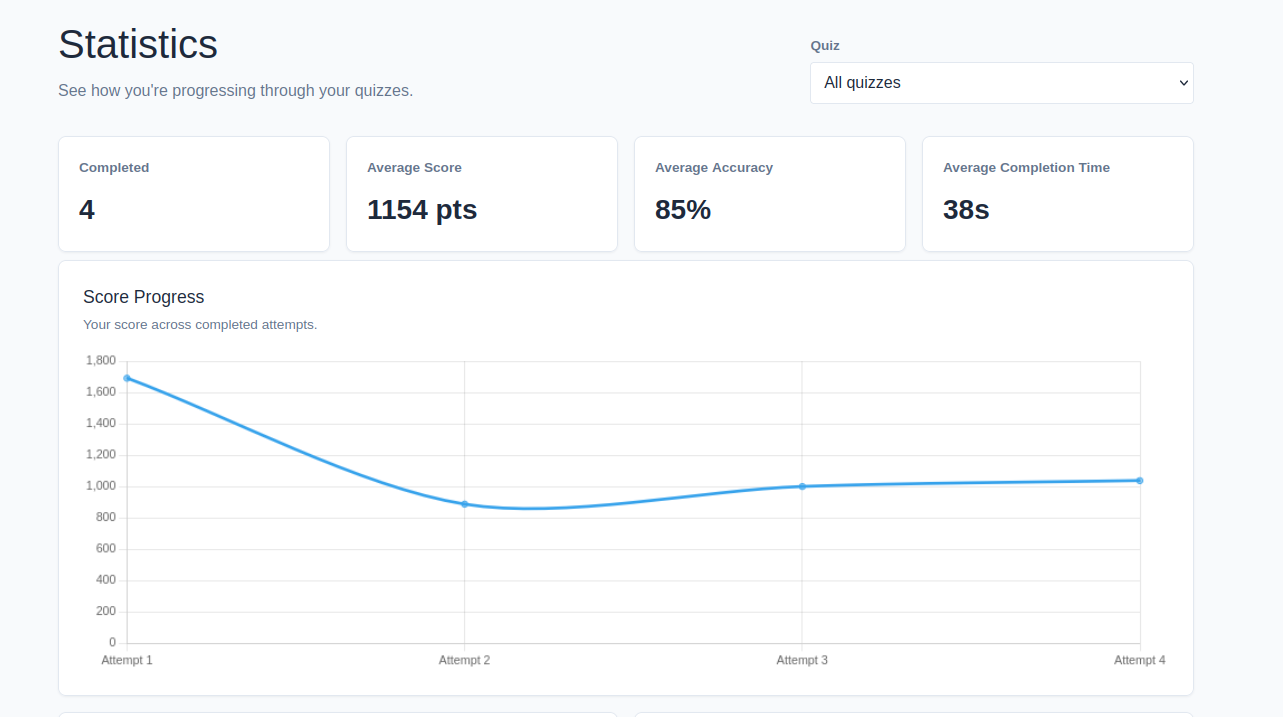
\includegraphics[width=15cm]{images/statistics1.png}
    \caption{Στατιστικά του χρήστη (1)}
    \label{fig:dashbord}
\end{figure}

\begin{figure}[htp]
    \centering
    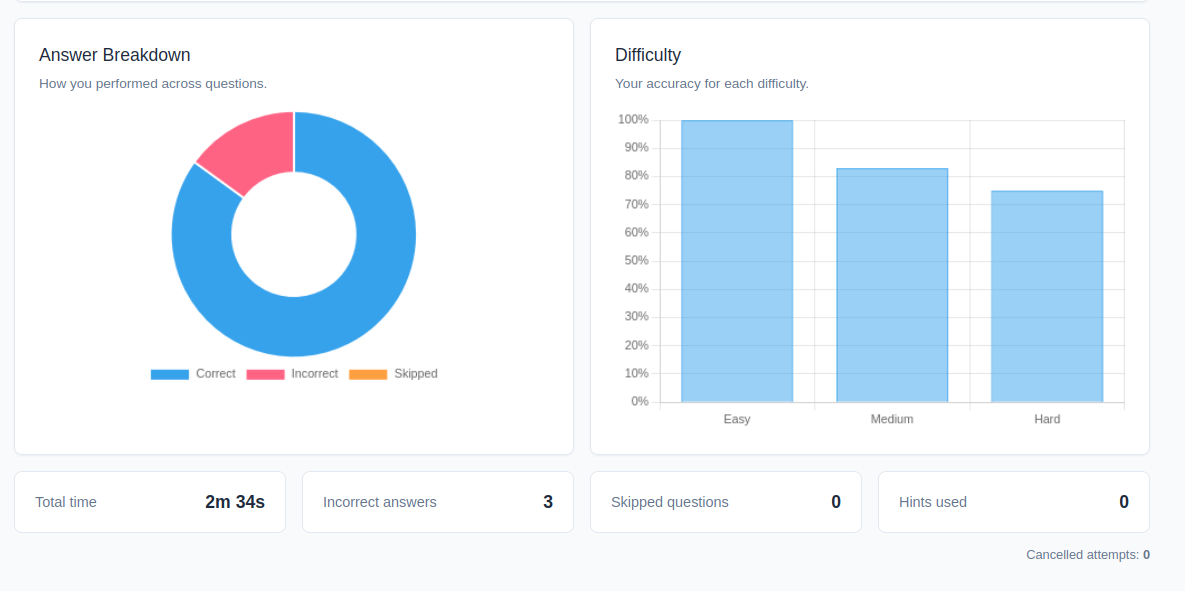
\includegraphics[width=15cm]{images/statistics2.png}
    \caption{Στατιστικά του χρήστη (2)}
    \label{fig:dashbord}
\end{figure}

\begin{figure}[htp]
    \centering
    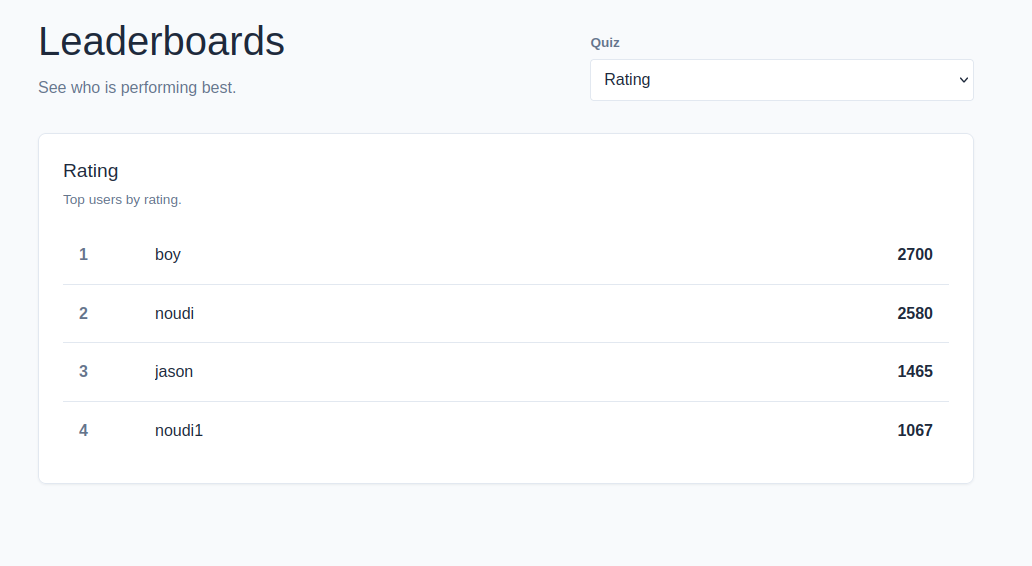
\includegraphics[width=15cm]{images/leaderboards total elo.png}
    \caption{Συνολικό \foreignlanguage{english}{Leaderboard}}
    \label{fig:dashbord}
\end{figure}

\begin{figure}[htp]
    \centering
    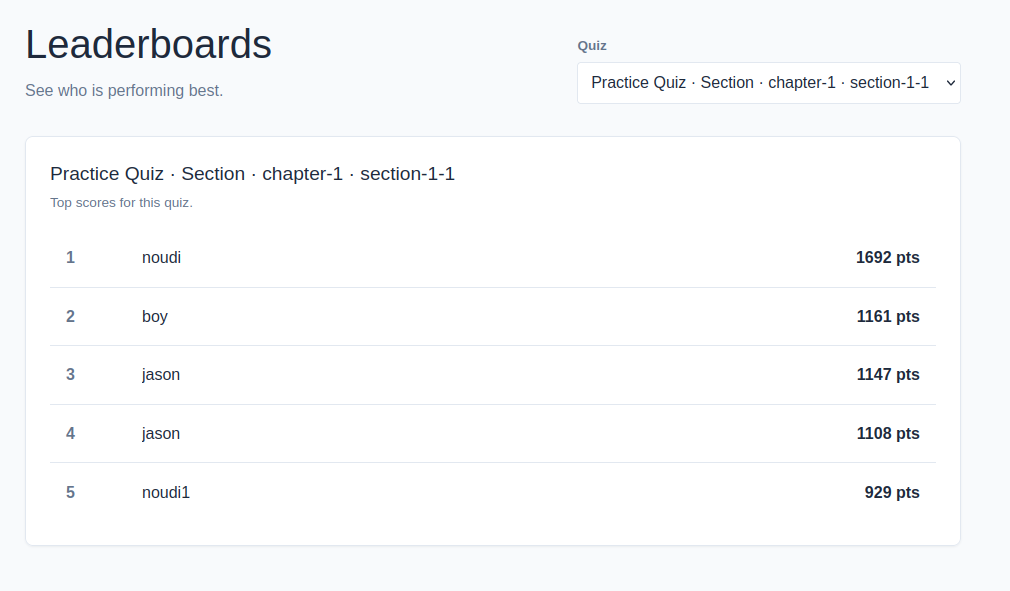
\includegraphics[width=15cm]{images/leaderboards section.png}
    \caption{\foreignlanguage{english}{Leaderboard} για το \foreignlanguage{english}{Quiz} της υποενότητας 1.1}
    \label{fig:dashbord}
\end{figure}

Το \foreignlanguage{english}{LeaderboardService} παρέχει δύο είδη κατάταξης. Όταν δεν έχει επιλεγεί συγκεκριμένο \foreignlanguage{english}{Quiz}, εμφανίζονται οι δέκα χρήστες με την υψηλότερη βαθμολογία κατάταξης \foreignlanguage{english}{(rating)}, όπως αυτή περιγράφηκε στην ενότητα "Βαθμολογία Κατάταξης". Όταν, αντίθετα, επιλεγεί ένα συγκεκριμένο \foreignlanguage{english}{Quiz}, το \foreignlanguage{english}{service} συγκεντρώνει τις ολοκληρωμένες προσπάθειες όλων των χρηστών για αυτό το \foreignlanguage{english}{Quiz}, υπολογίζει τη βαθμολογία τους μέσω του \foreignlanguage{english}{QuizResultService} και επιστρέφει τους δέκα χρήστες με την υψηλότερη επίδοση σε αυτό. Με αυτόν τον τρόπο, το \foreignlanguage{english}{Leaderboard} λειτουργεί συμπληρωματικά προς τη γενική βαθμολογία κατάταξης, επιτρέποντας στους χρήστες να συγκρίνουν την απόδοσή τους τόσο συνολικά όσο και ανά ενότητα ύλης.


\newpage
\listoffigures
\newpage

\section{Αναφορές}
[1] \foreignlanguage{english}{Chen, H.-M., Nguyen, B.-A., Chang, Y.-W., \& Dow, C.-R. (2024). \itshape{A gamified method for teaching version control concepts in programming courses using the GIT education game}. Electronics, 13(24), 4956.}\foreignlanguage{english}{https://doi.org/10.3390/electronics13244956}

[2] \foreignlanguage{english}{Helgesson, D., Appelquist, D., \& Runeson, P. (2021, July 9). \itshape{A grounded theory of cognitive load drivers in novice agile software development teams.} arXiv.Org.} \foreignlanguage{english}{https://arxiv.org/abs/2107.04254v1}

[3] \foreignlanguage{english}{Isomöttönen, V., \& Cochez, M. (2014). \itshape{Challenges and confusions in learning version control with git. Information and Communication Technologies in Education, Research, and Industrial Applications}, 178–193.} \foreignlanguage{english}{https://doi.org/10.1007/978-3-319-13206-8\_9}

[4] \foreignlanguage{english}{Kontogianni, A (2024, April 24).} \itshape{Σχεδιασμός Εκπαιδευτικού Λογισμικού}
[\foreignlanguage{english}{Course handout}]. \foreignlanguage{english}{TMD101}.

[5] \foreignlanguage{english}{Skinner, B. F. (1953). \itshape{Science and human behavior.} Macmillan.}

[6] \foreignlanguage{english}{Stack Overflow. (2022). Stack overflow developer survey 2022. Stack Overflow.}
\foreignlanguage{english}{https://survey.stackoverflow.co/2022/#overview}

[7] \foreignlanguage{english}{W3SCHOOLS. (n.d.). \itshape{Git tutorial. Www.W3schools.Com.} Retrieved September 8, 2026, from} \foreignlanguage{english}{https://www.w3schools.com/git/}

[8] \foreignlanguage{english}{Wagner, G., \& Thurner, L. (2025). \itshape{Teaching tip rethinking how we teach git: Pedagogical recommendations and practical strategies for the information systems curriculum.} Journal of Information Systems Education, 36(1), 1–12.} \foreignlanguage{english}{https://doi.org/10.62273/btkm5634}

[9] \foreignlanguage{english}{Watson, J. B. (2012). \itshape{Behaviorism}. Forgotten Books.}

\end{document}











